\chapter{Introduction}
\label{ch:introduction}

\section{The universe of particles}

The idea of understanding the physical world by identifying its
fundamental constituents is a very old one. Ancient eastern and
western philosophers independently attempted the feat, concluding
that the world could be reduced 
to ``elements'' such as water, earth, and fire.
As observational science became a more prominent component of modern thought, 
evidence mounted that these elements themselves were 
not indivisible. Perhaps the Greeks had not identified
the correct fundamental elements, but the belief that this endeavor could
be accomplished lived on.

A major attraction of identifying the fundamental building blocks of the universe
is the implication for constructing a macroscopic description from these
pieces. This process of understanding a complex system 
by reducing it to its essential components,
termed ``reductionism'' by philosophers, 
has formed the backbone of scientific endeavor for much of history.
In practice, the step from the fundamental to the macroscopic 
is far from trivial. Despite a well-established
understanding of the proton constituents and their interactions,
predicting the proton mass from first principles has only recently 
been achieved~\cite{Durr:2008zz}, and larger systems remain well
out of reach.
In addition to the challenges of calculability, additional structures
may arise from the nature of large systems, such as ferromagnetism or 
superconductivity.
This long-accepted path to a complete description of the physical world
has thus been called into question, and it may never be feasible
to achieve a theory of biology built from the findings of particle 
physics~\cite{Anderson393}.
Yet there is an undeniable elegance in achieving a concise description
of the fundamental elements of the natural world and their interactions,
and this remains the target of the field of particle physics today. 

For over a century, particle physics has been characterized by experimental
discoveries, many predicted by theoretical inferences, and others 
completely unexpected.
They have dramatically propelling the field forward,
while at times upending the accepted thought.
The history of particle physics is a fascinating one, with a subtle 
and intricate narrative justifying a much deeper discussion than presented
here. Ref.~\cite{Griffiths:2008zz} gives a technical introduction to the field in a historical
context, whereas Ref.~\cite{kragh2002quantum} gives a purely 
historical account. An encyclopedic overview of the major
theoretical and experimental advances in particle physics is given in Ref.~\cite{Ezhela:1996xi}.

The modern genesis of the field can reasonably be traced to 
the discovery of the electron in 1897 by J. J. Thomson~\cite{doi:10.1080/14786449708621070}, a particle still
believed to be elementary today.
At the time, though supported by the thermodynamic studies of Ludwig Boltzman,
the once-popular idea of a quantized unit of matter was
held in widespread doubt. 
The investigation of radioactive decays, by Becquerel,
Marie and Pierre Curie, and Rutherford, 
became closely linked with efforts to categorize
the structure of the chemical elements, assumed to be
building blocks of nature. 
However, as the atomic model became accepted, 
it quickly became clear that the atom itself is not elementary.

The subdivision of the atom into 

Discovery of the nucleus
Discovery of the proton
Discovery of the neutron

Forces needed to hold them together
Electromagnetic force


But the nucleus needs the strong force
But atoms also decay!
Nuclear decay -- weak force

The photon is spin 1 whereas the electron, proton, and neutron are spin 1/2.

\textbf{What points do I want to make?}
\begin{itemize}
  \item Introduce all the forces
  \subitem Electromagnetic + QM -- hold the atom together
  \subitem Strong -- holds the nucleus together
  \subitem Weak -- responsible for weak decays. It holds the atoms together
  \item The fact that quantum gauge theory can describe everything
  \item Other cruicial ideas
    \subitem Quantization of angular momentum, ``spin''
    \subitem Parity violation of weak decays
    \subitem Short range, weakness of the weak decay
\end{itemize}

A mathematical understanding of the electromagnetic interactions 
governing the interaction of the proton and electron had
already been established by James Clerk Maxwell decades before Thomson's work.
With the new quantum theory rapidly developing in the 1920s, the electromagnetic
interaction is also sufficient to explain the stability and arrangements of
electrons into atomic orbitals around the nucleus. 
Furthermore, the quantum theory provides a resolution of a seeming
conflict between the wave-like and particle-like nature of light.

The quanta of light, the photon, is now understood to communicate the electromagnetic force.
In fact everything is a wave particle

By the early 1940s, these pieces had evolved into the theory of quantum 
electrodynamics, the first
quantized theory of particles and their interactions in the language 
of quantum field theory. 

It can't explain, however, why the proton stays in one piece. For this you need the 
strong force.
You should probably introduce spin and the neutron here, if possible.

This would all be well and good, but it isn't the whole story! We know of weak 
decay, and we can't explain this. 
Its quite weird that it violates parity
\textbf{This will be a good chance to mention that more mathematical discussion will follow}

A unification of the electromagnetic and weak nuclear force was achieved
by Sheldon Glashow, Abdus Salam, and Steven Weinberg in the early 1970s.
A crucial component of their theory is the presence of a scalar field, 
which gives mass to the W and Z bosons through EWSB, leading to the 
short range of the weak force.
A description of the strong nuclear force as a quantum 
gauge theory followed,
with the inverse distance scaling properties of the theory,
termed quantum chromodynamics (QCD), demonstrated by
David Gross, David Politzer and Frank Wilczek.
The discovery of the gluon, the so-called gauge boson of the theory,
in 1979 at the Deutsches Elektronen-Synchrotron (DESY) in Hamburg, Germany
provided definitive confirmation
of gauge theory as the theoretical foundation of the particle physics.
The outstanding prediction of the 
electroweak theory, that the W and Z bosons which communicate the weak 
interaction acquire mass through the presence of scalar field, required
longer for experimental confirmation. This confirmation arrived a half-century
later, with the observation of the Higgs boson at CERN in 2012.
Together, the description of these interactions and the particle content
and these interactions described by the EW and QCD theories are known
as the standard model of particle physics.

Simultaneous to the efforts to develop a mathematical language to describe 
the fundamental particles and their interactions was an experimental effort 
to find and categorize them. 
An truly fundamental building block of nature is indivisible, therefore, it 
must be impervious to all attempts to break it into pieces.
Radioactivity gives crucial insights into this endeavor, as it represents
the spontaneous breakdown of atoms. However, as seen for $\beta$-decay,
the products of a decay are not necessarily the initial constituents.

\textbf{maybe introduce the weak decay here?}

\section{Particle scattering experiments}
In addition to studying the products of these decays themselves, 
Earnest Rutherford realized the energetic decay products of
radioactive nuclei could 
themselves be used as probes of other nuclei.
By directing the 
helium nuclei (referred to as $\alpha$ particles) emitted from radioactive radium decay towards gold foil
and measuring the deflection
angles, he and his collaborators demonstrated that the deflection
patterns of the scattered $\alpha$ particles were consistent with 
a concentrated positive charge at the center of atoms,
the atomic nucleus~\cite{Rutherford:1911zz}.
Inferring information about the properties and interactions of particles based on their
behaviour when scattered---referred to as a ``scattering experiment''---is still central 
to particle physics experiment today.

This thesis concerns measurements of \pp scattering. We focus on protons collided
at sufficiently high energy to overcome the electromagnetic repelling force 
to allow a direct interaction of the quarks and gluons that compose the protons.
Fig.~\ref{fig:scattering} gives a sketch of the scattering experiment approach
to the discovery of the Higgs boson production in \pp collisions with decays to two 
photons ($\gamma$). Protons of known energy and momentum are brought to collisions.
The outgoing particles---photons, in this example---are detected, and measurements 
of their properties, along with knowledge of the incoming particles, are used to infer
information about the unseen interaction. As discussed in Chapters~\ref{ch:phenomenology}
and \ref{ch:simulation}, such diagrams are not just useful visualizations of the 
interaction (in this case, the production and decay of the Higgs boson), they can be
connected to mathematical expressions used to predict explicit properties of
the outgoing particles. In this example, predictions of photon properties with
and without the existence of the Higgs boson can be compared to the experimental observation,
which conclusively favors the with-Higgs-boson scenario.

\begin{figure}[htbp]
  \centering
   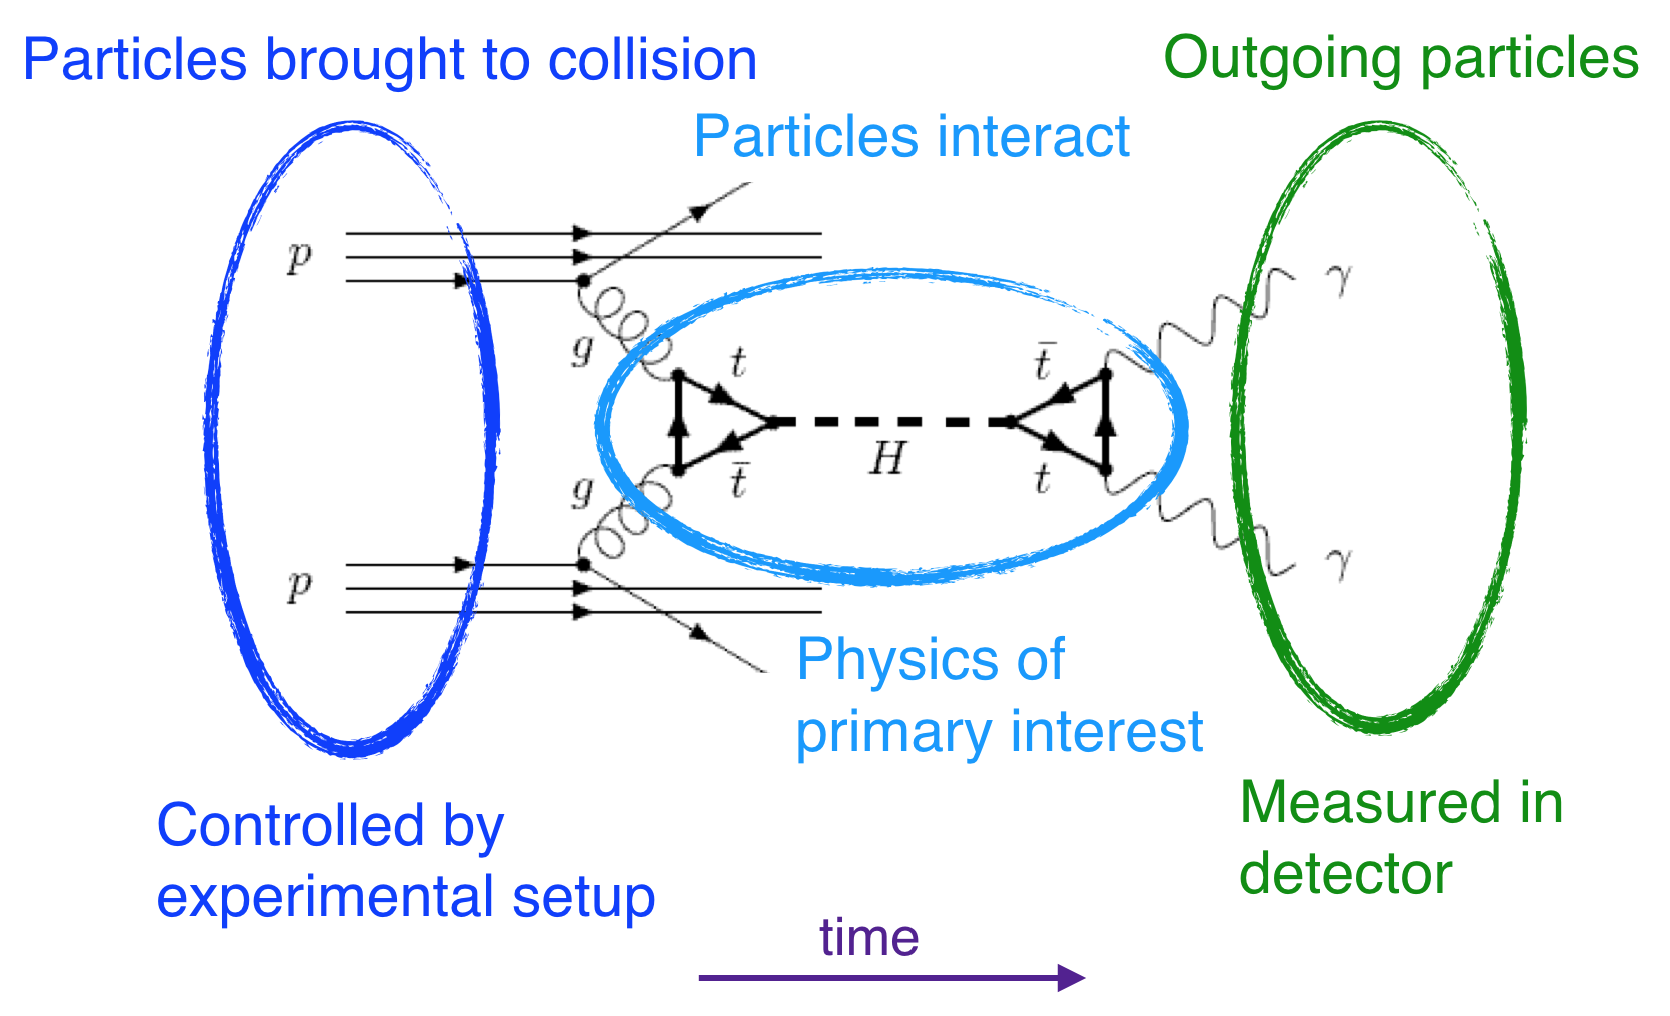
\includegraphics[width=0.9\textwidth]{figures/Chapter1/ScatteringExperiment.png}
  \caption{
    Illustration of Higgs boson production with decay to two photons 
    in a $\pp$ scattering experiment.
  }
 \label{fig:scattering}
\end{figure}

Because high-energy particle interactions are driven by quantum mechanics, they are stochastic
in nature. Therefore, a single collisions cannot be uniquely interpreted in terms
of a given interaction (or ``process''). Rather, features of a measured process,
such as the consistency or inconsistency with a hypothetical interaction or the presence
of a new particle, must be inferred from collective results.
To this end, a critical metric of scattering processes is the scattering cross section.
For a particle beam scattered off a target, or equivalently, two beams of particles
brought to collision, the cross section is the effective area of the beam
deflected by scattering from the target (or other beam). For two beams with 
densities $\rho_{\mathcal{A}}(x)$, $\rho_{\mathcal{B}}(x)$ and length $\ell_{\mathcal{A}}$, 
$\ell_{\mathcal{B}}$, the cross section is defined as~\cite{Peskin:1995ev}
\begin{equation}
  \sigma = \frac{\text{Number of scattering events}}
    {\ell_\mathcal{A}\ell_\mathcal{B}\int\mathrm{d}^2x\rho_{\mathcal{A}}(x) \rho_{\mathcal{B}}(x)}\,.
  \label{eq:crossSection}
\end{equation}
For example, the cross section $\sigma_{\pp\to\EE}$ relates the number of 
events with two electrons produced in the scattering of two proton beams.
The cross section is only unambiguously defined experimentally when it relates
only the initial state and final state. 
However, it is common to discuss the cross section
for, e.g., Higgs boson production, under the assumption that an theoretical extrapolation
has been made in order to connect the measured particles (e.g., photons) to their production
mechanism.

It is also often useful to discuss not just the total cross section for all scattering to a final
state, but to consider a \emph{differential cross section}, dependent on properties
of the final state particles. For example, the differential cross section 
$\mathrm{d}\sigma_{\pp\to\EE}/\mathrm{d}E_\Pem$ is measured by dividing 
the number of scattering events by properties of the outgoing electron energy $E_\Pem$
to produce a differential distribution of the production rate in terms of $E(\Pem)$.
A measurement may also be restricted to consider only the scattering of outgoing particles
into a specific geometrical region or above some threshold energy and momentum. Such a measurement
is termed a \emph{fiducial cross section}, restricted to a fiducial phase space
defined by the geometrical and kinematic restrictions of the measurement.

\section{Particle colliders}
Rutherford continued to use the radioactive decays of elements as a means
for particle scattering measurements through the early 1900s. Yet it was clear that
a means of accelerating collisions to higher energies would be needed
to continue to probe the structure of the nucleus.
This requirement lead to the invention of
the first particle accelerators, which have come to define the field ever since.
An electrostatic accelerator was developed at the Cavendish Laboratory
in Cambridge, England by John Crockcroft and Ernest Walton and
was used to split Lithium into Helium atoms in 1932~\cite{CrockcroftWalton}.
Concurrently, Ernest Lawrence developed the cyclotron in California~\cite{PhysRev.40.19},
which became a model for many future accelerator facilities.
These inventions triggered an explosion in the field, marked by a continual 
effort to collide particles at higher and higher energies. 

New equipment for detecting these particles,
such as the cloud chamber developed by Charles Wilson
in 1911~\cite{doi:10.1098/rspa.1912.0081}, 
was being developed concurrently. The cloud chamber emerged as a powerful
tool for the characterization of radiatactive decay, 
and opened our eyes to the radiation bombarding the earth from
outside the atmosphere. The discovery of the positron, the first

As well as the muon, evidence for generations of matter.

\begin{itemize}
  \item The muon, equated with generations
  \item So are strangeness and charm
  \item The gluon is important for realizing that the gauge theory can also be applied to the strong force
\end{itemize}

By the 1950s, particle physicists were faced with a ``particle zoo''
of seemingly fundamental objects spanning a huge range of masses. 
An underlying structure of the properties of many of these particles, 
now known as hadrons, was described by Murray Gell-Man and George Zweig in 1964.
They realized the properties of the many observed hadrons could be 
attributed to combinations of different elementary particles,
which Gell-Man termed quarks.
Whether these particles were physical entities or abstractions was 
not immediately evident, but experiments at the Stanford Linear Accelerator
at the end of the 1960s showed the proton to have point-like constituents
with the properties Gell-Man and Zweig predicted.

Despite the progress in explaining the structure of hadronic matter,
it remained unclear that the language of a quantum gauge theory, 
so successful in the formulation of the electromagnetic interaction, could 
also describe the strong nuclear force responsible for the formation
of these composite particles, and the weak nuclear force responsible for
a subset of their decays. Both exhibited striking differences with
respect to the electromagnetic interaction:
the weak nuclear force acts over a much smaller distance, while
the strong nuclear 
force has an inverted scaling with distance, increasing at higher separation
of the interacting objects while decreasing at very short ranges. 

\textbf{You need to connect the particle zoo to the idea of hadrons, quarks, and gluons}

\textbf{The point here is the weak force, a unification of the EM and W.}
\textbf{You want to introduce the stuff you work on, as well as the point that one mathematical framework works.}

Many major discoveries
are closely linked with technological advancements and collaborative
efforts leading to more powerful accelerators.
The facilities at the European Center for Nuclear
Research (CERN), DESY, and at the 
Fermi National Accelerator Laboratory (Fermilab) in Illinois
are strongly associated with the 
discoveries they enabled, including: evidence for the force carries
of the EW and QCD interactions, the {\PW} and {\PZ} bosons~\cite{},
the gluon at PETRA collider at DESY by the TASSO experiment~\cite{},
and the discovery of the top quark by the D0 and CDF Collaborations
at the Tevatron at Fermilab~\cite{}.

The most powerful collider ever built, the Large Hadron Collider (LHC) at CERN,
now allows the study of the most energetic particle collisions ever
recorded in the laboratory, reaching concentrated energies only replicated
in the most cataclysmic events in the universe. The LHC
was planned, developed, and built over the course of decades, with
personnel and funding from countries throughout the world.
It accelerates proton beams to energies of 
$6.5\times10^{12}$ terra-electronvolts (TeV),
where $1\unit{eV}=10^{-12}\TeV=1.602\times10^{-19}\unit{J}$, that are brought to collisions at 
a center-of-mass energy $\sqrt{s}=13\TeV$.

In addition to accelerating protons to groundbreaking energy, the LHC
delivers a very high rate of \pp collisions. This allows very rare 
interactions to be studied,
and is critical to obtaining statistically significant results.
In modern particle scattering experiments, the beam is not continuous,
as suggested by Equation~\ref{eq:crossSection}. It is helpful
to express the properties of the beam particle density and effective length 
in terms of the luminosity $\mathcal{L}$ which captures the geometric properties of
the beam such that
\begin{equation}
  \text{Number of scattering events} = \sigma\mathcal{L}\,.
\end{equation}
This work is based on studies of pp collisions delivered by the LHC 
and collected by the Compact Muon Solenoid detector in 2016, which 
are discussed in detail in Chapter~\ref{ch:lhcAndCMS} of this thesis.
The precise definition of the luminosity for this experiment will also be
discussed.

\section{The particle content of the standard model}

The experimental and theoretical work discussed here,
as well as many other successful discoveries, measurements, and 
breakthroughs---combined with many more null results and
unfulfilled hypotheses---have lead to the modestly-named 
standard model (SM) of particle physics.
With the discovery of the Higgs boson, the SM is widely considered to 
be complete.
\textbf{What are some shortcomings?}

The currently known particle content of the universe is depicted in Fig.~\ref{fig:theparticles}.
The quarks, highlighted in green, and leptons, highlighted in purple,
form matter, while the vector bosons, highlighted in red, mediate the 
interactions of this matter. The Higgs particle, shown in yellow,
has a unique role in the SM. It arises from the Higgs field, which
leads to masses for the W and Z bosons as well as the quarks and leptons.
The underlying mathematical framework used to understand the quantum 
properties of these particles and their interactions will be further discussed
in Chapter~2. 

\begin{figure}[htbp]
  \centering
   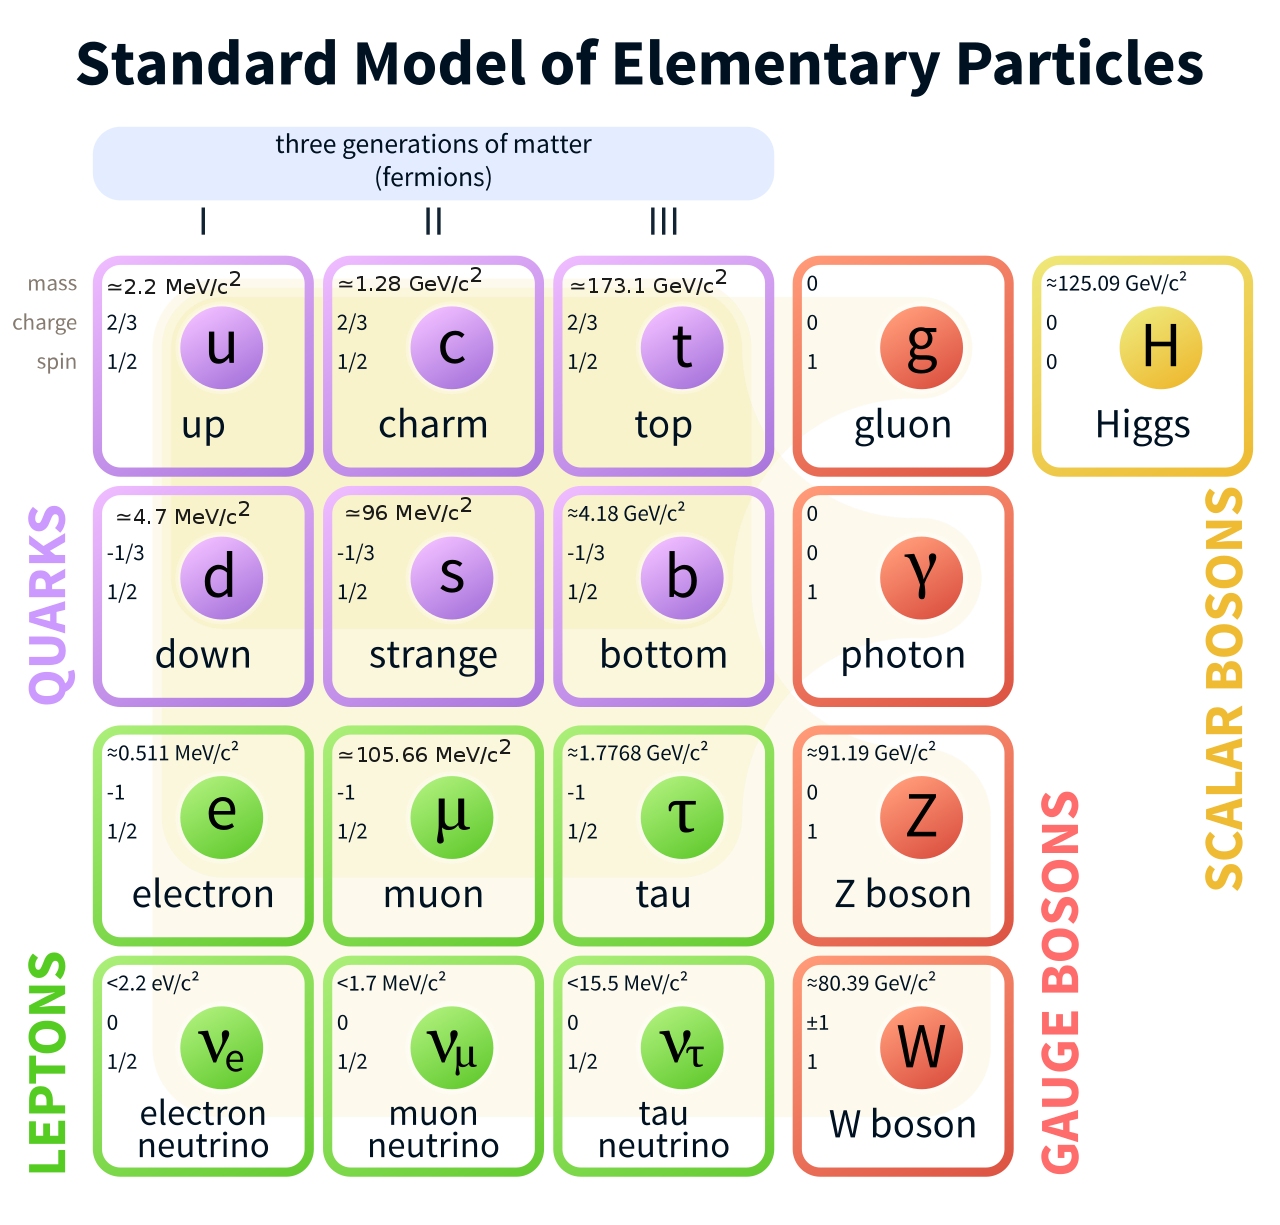
\includegraphics[width=0.9\textwidth]{figures/Chapter1/ChartOfParticles.png}
  \caption{
    The experimentally established particle content of the universe.
  }
 \label{fig:theparticles}
\end{figure}

Basically, follow Nate here.

fermions are spin 1/2, they compose matter
What are they?

Leptons interact via the electroweak force.
They carry what electric charge?
Partity is a defining feature of the weak force. Only leptons
with left-handed helicity interact via the weak force, whereas
all interact with the electromagnetic.

Quarks interact via both the electroweak and strong force.
Quarks form bound states of hadrons, e.g., the proton and neutron.

Interactions in the SM are communicated by the spin 1 bosons.
The W and Z bosons communicate the weak force, whereas the photon
communiciates the electromagnetic portion.

The role of the Higgs boson will be discussed more in Chapter 2.


\section{Overview}
This thesis presents measurements of the production of events
Events with 
three leptons, two forward ``jets'' of clustered hadronic particles,
and an imbalance of transverse momentum are selected to 
isolate contributions involving the simultaneous
production of a $\PW^{+}$ or $\PW^{-}$ and a $\PZ$ boson, the heavy particles
that communicate the weak force.
Selected events are used
to measure the rate of production of processes predicted by the standard
model (SM) of particle physics, the most complete theoretical expression
of the known particles and forces of the universe, and to search for hypothetical extension
of the SM. 

A dedicated search
for a rare, previously unobserved SM process, referred to as electroweak (EW)
WZ production (referred to as \EWWZ production), is presented. 
The presence and production rate of the \EWWZ process is intimately connected to the 
mathematical structure of the weak interaction, which predicts self-interactions
of the massive vector bosons,
and the phenomenon of EW symmetry breaking (EWSB) \cite{Quigg:2009vq}.
A fundamental prediction
of EWSB, fulfilled in the standard model (SM) by the Brout-Englert-Higgs (BEH) 
mechanism~\cite{PhysRevLett.13.321,Higgs:1964ia,PhysRevLett.13.508,PhysRevLett.13.585,PhysRev.145.1156,PhysRev.155.1554},
is the emergence of a scalar particle known 
to as the Higgs boson. 
This particle was first observed by the 
ATLAS~\cite{Aad:2012tfa} and CMS~\cite{Chatrchyan:2012xdj,Chatrchyan:2013lba} Collaborations
at CERN in 2012, providing compelling evidence for the BEH mechanism as
a component of the SM theory.
The triple and quartic self-interactions of the vector bosons, 
and their couplings of 
the massive vector bosons to the Higgs field---which depend on the 
Higgs boson {\PH} mass---are exactly predicted in the SM.
Physics beyond the SM in the EW sector is expected to include 
interactions with the vector and Higgs bosons that modify their effective couplings. 
Characterizing the self-interactions of the 
vector bosons is thus of great importance. 

This thesis presents the first study of this process performed by 
the CMS Collaboration~\cite{Sirunyan:2019ksz}.
Selected events are used to place constraints on physics beyond the SM (BSM) in terms
of explicit models predicting charged Higgs bosons, decaying to a $\Wpm$ and a $\PZ$
boson, and on generalized models of new interactions modifying
in the rate of production, or in kinematic distributions, of selected events.

The outline of this work is as follows: Chapter~2 presents an extended 
overview of the theoretical underpinnings of this work, including the foundations
of the SM and the role of \EWWZ production in this framework. The motivations 
and structure of SM extensions probed in this work are also introduced.
Chapter~3 introduces the experimental setup and apparatus used to study W and 
Z boson production in the laboratory. The LHC and the Compact Muon Solenoid 
detector are presented and discussed. Chapter~4 describes the procedure of 
building predictions for vector boson production in pp collisions.
The use of these predictions in interpreting results, and in developing simulation
of particle production and decays in pp collisions including their interactions
with the detector -- which are used 
guide the analysis approach and optimizations -- are discussed. Chapter~5 presents
the process of finding particle candidates from electronic signals in the detector.
Chapter~6 details the procedure of this analysis and the statistical underpinnings
used to extract results. Chapter~7 discusses the results obtained from this study
including interpretations and implications. Chapter~8 summarizes the
results presented and discusses future extensions.
